\documentclass[a4paper,10pt,twocolumn]{article}
	\usepackage{amsmath}
	\usepackage{graphicx}
	\usepackage{newtxtext,newtxmath}
	\usepackage{lipsum}
	\usepackage{tabularx}
	\usepackage{booktabs}
	\usepackage{algorithm}
	\usepackage{algorithmic}
	\usepackage{float}
	\usepackage{geometry}
	\usepackage{draftwatermark}
	\usepackage{titling}
	\usepackage{makeidx}
	\usepackage{url}
	\usepackage[title,titletoc]{appendix}
	\setlength{\parindent}{0pt}
	\SetWatermarkText{}
	\SetWatermarkScale{1}
	\geometry{
	a4paper,
	total={170mm,257mm},
	left=20mm,
	top=20mm,
	}
	\frenchspacing
	\renewcommand{\appendixname}{Appendix }
	\pretitle{%
	\begin{center}
	\LARGE
	
\includegraphics[width=40mm]{logo-min}\\[\bigskipamount]
	Aidos Kuneen \\ 
	\Large
	}
	\posttitle{
		\normalsize
		\end{center}}
	
	
	
	\title{--- A Blockless and Anonymous Cryptocurrency for the Post-Quantum Era ---}
	
	\author{
		Aidos Developer \and Aidos Foundation
	}
	\date{January, 2018 \\ Version 0.04 (DRAFT)}
	
	\begin{document}
	
	\twocolumn[
		\maketitle
	
	\begin{abstract}
			In this white paper we introduce a new cryptocurrency, \emph{Aidos Kuneen}. Aidos Kuneen has been developed to deliver 
			a fast, anonymous, blockless, decentralized and scalable solution for post-quantum era transfers with zero fees. 
	
	\vspace{2.5mm}
			
			Aidos Kuneen employs a mechanism known as \emph{iMesh}, within iMesh all transactions are directly referenced by
			one another in order to form a \emph{Directed Acyclic Graph (DAG)} structure.
	
	\vspace{2.5mm}
			
			The inclusion of `SPECTRE' allows full-nodes to determine which transactions are legitimate within the DAG structure 
			and to reject those that are not. In addition, SPECTRE provides resilience against any attackers who may happen to gain 
			control of up to 50\% of the network's computational power.
	
	\vspace{2.5mm}
			
			To ensure continued security in the post-quantum era, Aidos Kuneen utilises the hash-based signature `XMSS'. XMSS
			provides for both a small signature and a small public key size which in turn reduces network load.
	
	\vspace{2.5mm}
		
			In order to provide anonymity within the network, Aidos Kuneen employs \emph{AKShuffle}. AKShuffle 	
			incorporates the post-quantum, zero-knowledge proof `ZKBoo (ZKB++)', this allows for truly anonymous transfers 
			throughout the entire network.
	
	\vspace{2.5mm}
			
			To allow Aidos Kuneen to service the expected future growth of the `IoT' sector we introduce an innovative new 
			co-operative Proof of Work mechanism known as \emph{coPoW}\@. coPoW allows a number of senders within the network to 
			co-operatively perform the necessary Proof of Work in order to confirm transactions on the network, thus reducing 
			the physical processing requirements of any one sender.
	
	\vspace{2.5mm}
	
			Finally, we provide a simulation of the number of leaves in iMesh and we further determine the minimum number of 
			reference transactions required in order to converge the DAG and deliver fast confirmation times, whilst still having minimal effect on the transaction size.
			
			\end{abstract}
	
			\vspace{1.5cm}
	
	\footnotesize
	Copyright \copyright  2017--2018 by Aidos Developer and Aidos Foundation.
	
	\vspace{2mm}
		
	IN NO EVENT SHALL THE AUTHORS OR COPYRIGHT HOLDERS BE HELD LIABLE FOR ANY CLAIM, DAMAGES OR OTHER
	LIABILITY, WHETHER IN AN ACTION OF CONTRACT, TORT OR OTHERWISE, ARISING FROM,
	OUT OF, OR IN CONNECTION WITH THIS DOCUMENT, OR THE USE OF OR OTHER DEALINGS WITH
	THIS DOCUMENT\@.\\
	
	This work is licensed under a Creative Commons Attribution 4.0 International License. \\
	\url{http://creativecommons.org/licenses/by/4.0/} \\
	
\includegraphics{cc}
	]
	
	\normalsize
	\twocolumn[
	\tableofcontents
	\listoffigures
	]
	
	\clearpage
	
	\section{Introduction}
	Bitcoin, the once obscure cryptocurrency introduced by Satoshi Nakamoto~\cite{btc} in 2008, has now begun to draw much wider attention 
	from both the general public and governments alike. Within the Bitcoin network, transactions are written into `blocks', these blocks 
	are then cryptographically validated by powerful computers known as `miners' using a Proof of Work (PoW) system. Once a block has been 
	validated it is then appended to the end of a continually growing chain of blocks aptly named `the block-chain'. Miners are 
	subsequently rewarded for successfully validating a block by means of the transaction fees paid by senders who transact on the Bitcoin 
	network.\\
	
	Currently, blocks are added to the blockchain at a rate of approximately one every 10 minutes. The transactions contained within the
	blocks consist of both input and output addresses, with the inputs themselves being the outputs of previous transactions --- this 
	provides an auditable history of all past Bitcoin transactions within the network. In order to prove ownership, transactions are signed 
	by the address owner with an Elliptic Curve Digital Signature Algorithm (ECDSA).\\
	
	However, in recent years a number of problems have been identified with the Bitcoin implementation, including:
	\vspace{-0.5\baselineskip}
	\begin{itemize}
		\setlength\itemsep{0em}
		\item\textbf{Limited Scalability}\mbox{}\\ 
		Within the core Bitcoin code, the maximum block size is restricted and blocks are unable to store transactions once this limit 
		is exceeded. This in turn leads to a scalability problem when many transactions are broadcast simultaneously with many of them 
		being unable to be included in the current block.
		\item\textbf{High Transaction Fees}\mbox{}\\ 
		Senders are required to pay a transaction fee in order to incentivise the miners to include their transaction in a block.
		If Bitcoin usage continues to grow and the price of Bitcoin increases, the relative value of the fee will also increase.
		It no longer makes sense to send small transactions via the Bitcoin network
		as the fee could easily exceed the value of the Bitcoin being transacted. This forces senders to use complicated schemes to send small value transactions (e.g. 
		micropayment channels).
		\item\textbf{Poor Resistance Against Quantum Computers}\\ 
		As of 2017, the development of quantum computers is still in its infancy. However, experiments have already been carried out in 
		which quantum computational operations were executed on a small number of quantum bits. Furthermore, Google has reported its 
		intent to commercialize quantum technologies within the next five years~\cite{google}. At the same time, according to Shor's 
		algorithm~\cite{shor}, all algorithms based on the discrete logarithm problem (including ECDSA as used in 
		Bitcoin), can be easily solved with a sufficiently powerful quantum computer. 
		\item\textbf{Limited Anonymity}\mbox{}\\ 
		The auditable nature of Bitcoin means that in order to spend Bitcoin, the spending transaction must refer back to the founding
		transactions that came before it, these founding transactions are open to the public. As such, anyone is free to track the flow
		of BTC from address to address.
	\end{itemize}
	
	In order to address these issues, we introduce a new cryptocurrency, \emph{Aidos Kuneen}.
	The Aidos Kuneen network, known as \emph{iMesh}, is based on \emph{Directed Acyclic Graph (DAG)} technology.
	In iMesh, transactions are directly referred to by other transactions and as such there are no blocks, and by extension, no block-chain.
	The confirmation of a transaction is determined by the number of other transactions which \emph{vote} for the transaction. In iMesh, we are able to achieve the benefits of scalability while completely removing the requirement for miners, which subsequently removes the need for the associated transaction fees that were once required in order to incentivise mining.
	
	\vspace{2.5mm}
	
	Adios Kuneen has been specifically designed to provide:
	\vspace{-0.5\baselineskip}
	\begin{itemize}
		\setlength\itemsep{0em}
		\item\textbf{Increased Scalability}\mbox{}\\ 
	In iMesh, one performs relatively simple PoW computations to confirm the transaction. After the transaction is broadcast to the network,
	the transaction is stored into iMesh immediately. Hence, there is no need to wait for one's own transaction to be stored. Additionally 
	there is no limitation to the size or number of transactions that can be stored at a time. The more iMesh grows, the greater the number 
	of transactions that become involved. This means that the confirmation time of any single transaction will reduce as the network matures.
	
	\item\textbf{Zero Fees}\mbox{}\\ 
	As one is no longer required to pay any transaction fees (owing to the fact that there are no miners), one is free to 
	transact with any amount, no matter how small without requiring any special knowledge or techniques.
	
	\item\textbf{Post-Quantum Resistance}\mbox{}\\ 
	In Aidos Kuneen we have specifically chosen a hash-based signature which provides strong post-quantum security. There have been a 
	number of different signature architectures developed to provide resistance to future quantum based computer hardware, including 
	Ring-LWE, Lattice and hash-based methods. However, the majority of these are not practical for our purposes due to their large key and 
	signature sizes. For example, the key sizes of Ring-LWE and Lattice based signatures weigh in at a number of kilobytes. This means that 
	if we were to employ one of these methods for example, we would be forced to use long alphanumeric address strings which are not 
	conducive to usage by the non-technical, general public. For a cryptocurrency that is intended for widespread daily use this is 
	completely unsuitable.
	
	\vspace{2.5mm}
	
	As such, we focus our attention on the family of hash-based signature methods instead. Some hash based functions 
	such as `SPHINCS', provide us with the ability to reuse the same public key multiple times, which is a step in the right direction. 
	However, SPHINCS also suffers from the same large public key size (around 1 kilobyte) as the other methods, again making it unsuitable 
	for our application. Eventually, the `eXtended Merkle Signature Scheme' (XMSS) was identified as being the ideal balance of human 
	usability and small key size. XMSS allows us to repeatedly utilise the same public key a large number of times (1000 times or more). 
	However, unlike SPHINCS, XMSS has a lightweight public key of only 32 bytes and a signature key size of approximately 3 kilobytes. By utilising XMSS we also benefit from \( 2^{128} \) bit post-quantum security~\cite{recom}.
	
	\item\textbf{Strong Anonymity}\\ 
	In order to achieve anonymity, we utilize the post quantum, zero-knowledge, non interactive (ZKNI) proof `ZKBoo' as presented 
	in~\cite{zkboo}. ZKBoo allows one to transact freely across iMesh, without the need to reveal one's address to either the receiver or to the wider network.
	\end{itemize}
	
	\section{Related Works}
	
	{\bf Monero\footnote{http://monero.org/}, Bytecoin\footnote{https://bytecoin.org/} and Zcoin\footnote{https://zcoin.io/}}
	
	To achieve anonymity, both Monero and Bytecoin use `ring signature' methods as discussed in CryptoNote~\cite{ringsig}.
	Ring signature methods rely on a signature which utilises a novel trapdoor function (e.g.\ public key encryption), unfortunately though, this feature is 
	not found in any of the available hash-based signature methods. Zcoin utilises a zero-knowledge, non interactive proof called `zk-SNARKs', however, zk-SNARKs is not quantum secure, owing to the fact that it uses pairing-based 
	cryptography\footnote{post-quantum Zcash (https://github.com/zcash/zcash/issues/805)}. 
	\\
	
	\noindent
	{\bf CoinJoin\footnote{https://en.bitcoin.it/wiki/CoinJoin}}
	
	Another potential option for providing anonymity, would be to use `CoinJoin' or one of its variants (e.g.\ `CoinShuffle'). However, 
	CoinJoin requires the presence of active participants at the same time one intends to send coins. This requirement could prove to be a 
	handicap in the early stages of adoption when the Aidos Kuneen userbase is still small. 
	\\
	
	\noindent
	{\bf IOTA\footnote{https://iota.org/}}
	
	IOTA is a DAG based, fee-less, IoT focussed cryptocurrency.
	
	IOTA is unique in that it makes use of ternary based signatures rather than standard binary. This is due to the fact that ternary based 
	systems are theoretically more computationally efficient than binary based systems. In Aidos Kuneen we have chosen to utilise 
	traditional binary based signatures in order to fully utilize existing CPU features (such as SIMD instructions and dedicated SHA 
	extensions). This decision was made because we believe that current generation digital processors are already sufficiently fast and 
	efficient enough to meet our requirements, with some IoT oriented processors already containing dedicated circuits for 
	SHA-2 based hash processing, e.g.~ARM processors\footnote{https://static.docs.arm.com/ddi0501/f/DDI0501.pdf}. We also believe that at 
	least in the short to medium term, binary based systems will continue to remain the dominant form for consumer grade hardware.
	
	\vspace{2.5mm}
	
	IOTA's confirmation process, as outlined in IOTA's white paper, counts only the number of referring transactions 
	(descendant transactions), we notice that as the total number of leaves in the DAG increases (as will occur naturally), 
	the percentage of these leaves to which descendant transactions refer will decrease.
	This means that attackers could potentially grow their malicious
	transactions faster than the network. To combat this we introduce a confirmation process based on \emph{SPECTRE} as presented 
	in~\cite{spectre}. In SPECTRE one does not only count the number of descendant transactions, but one also counts the number of other 
	transactions which subsequently vote for the transaction. Hence, even if the leaves do diverge, it is difficult for an attacker to grow 
	the confirmations of their malicious transactions.
	
	\vspace{2.5mm}
	
	Within the SPECTRE voting process, we still require faster DAG convergence for rapid confirmations. The white paper as presented by the 
	IOTA team does not specifically clarify the convergence behaviour of the DAG, rather the white paper simply states that `One 
	\emph{expects} that the \( L(t) \) (total number of leaves) remains stable'. As such, in Section 9, we additionally simulate the behavior of leaves within iMesh in order to ensure that the DAG converges.
	
	\section{Signature Scheme}
	\label{sec:sig}
	
	As previously mentioned, Aidos Kuneen employs XMSS as described in the RFC draft of IETF~\cite{ietf} as its signature algorithm. XMSS 
	itself is based on the earlier work of the Winternitz One Time Signature (WOTS+). WOTS+ is a hash based signature scheme designed for 
	single use only, XMSS builds upon this work and delivers a mechanism which makes it possible to sign multiple messages with a single 
	key.
	
	\subsection{WOTS+}
	
	\begin{figure}[ht]
		\begin{center}
		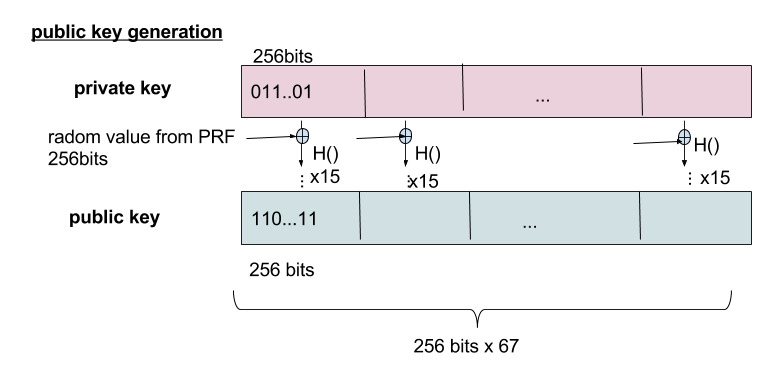
\includegraphics[width=80mm]{wots_pub.png}
		  \caption{Generation of the WOTS+ public key}
		\label{fig:wots_pub}
		\end{center}
	 \end{figure}
	
	\vspace{-3.5mm}
	
	 Figure~\ref{fig:wots_pub} demonstrates how a public key is generated. In order to generate a public key, one initially generates a series of 67 character strings consisting of 32 byte (256 bit) random binary data which becomes the 
	 private key \( Priv_{j}, j=1 \ldots 67\). Then, each \( Priv_{j} \) is hashed with the SHA-256 algorithm for a total of 15 passes. 
	 While hashing, each \( Priv_{j} \) is XORed with a value from a PRF (Pseudo Random Function). This XOR operation is employed to reduce 
	 the signature size while maintaining the same security level. The output of these operations becomes the public 
	 key \( Pub_{j}, j=1 \ldots 67\) which is also a 67 character string consisting of 32 byte binary data.
	
	 \begin{figure}[ht]
		\begin{center}
		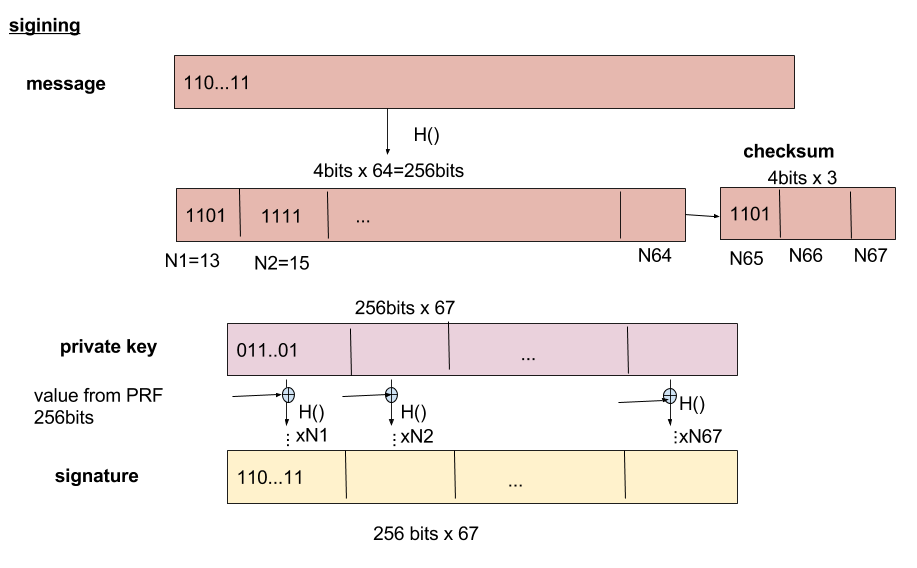
\includegraphics[width=80mm]{wots_sign.png}
		  \caption{Signing with the WOTS+ private key}
		\label{fig:wots_sign}
		\end{center}
	 \end{figure}
	
	\vspace{-3.5mm}
	
	
	 Figure~\ref{fig:wots_sign} illustrates how the message is signed. When signing, one calculates a 256 bit hash \( H(msg) \) of the original message, and a corresponding 12 bit checksum from \( H(msg) \).
	 Next, a series of 4 bit, 67 character binary strings \(N_i,i=1 \ldots 67\)  are produced from the \(H(msg)\) and the checksum. 
	 Each of the \( Priv_j \) values are then hashed for \(N_i\) times and XORed with the same 
	 values as used for \( Pub_{j} \), to produce the signature \( Sig_j, j=1 \ldots 67 \). 
	
	\vspace{2.5mm}
	
	The checksum is used to prevent 
	 attacks from malicious messages. For example, if there were no checksum and an attacker were to create a message whose hash were 000 
	 \ldots 0, i.e. \( N_i = 0, i=1 \ldots 64 \), then the signature would be equal to the private key and thus the private key would be 
	 exposed.
	
	 \begin{figure}[ht]
		\begin{center}
		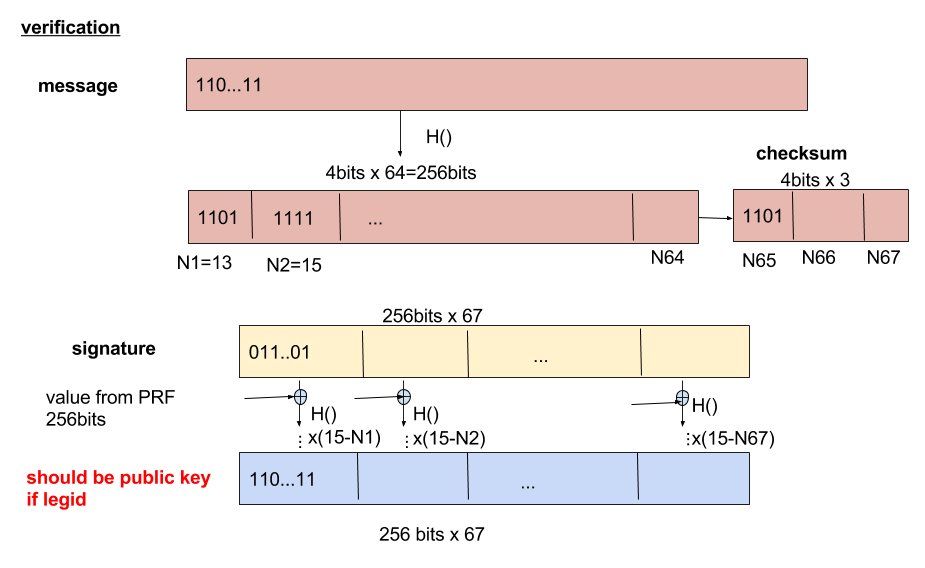
\includegraphics[width=80mm]{wots_veri.png}
		  \caption{WOTS+ Verification}
		\label{fig:wots_veri}
		\end{center}
	 \end{figure}
	
	\vspace{-3.5mm}
	
	 Figure~\ref{fig:wots_veri} illustrates how the signature is verified. In order to verify a signature, a verifier first calculates \(N_i, i=1 \ldots 67 \) using the same procedure for signing as explained 
	 above. Next, each \( Sig_j \) is hashed (\(15-N_i\)) times and XORed with same values as were used to produce \( Pub_{j} \). The output 
	 of which yields \( Pub'_j , j=1 \ldots 67\). This is then checked to confirm that it equals the signer's public key \( Pub_j,  j=1 
	 \ldots 67 \).
	
	\newpage
	
	\subsection{XMSS}
	
	Figure~\ref{fig:xmss_pub} demonstrates how the public key for XMSS is generated.
	
	\begin{figure}[ht]
		\begin{center}
		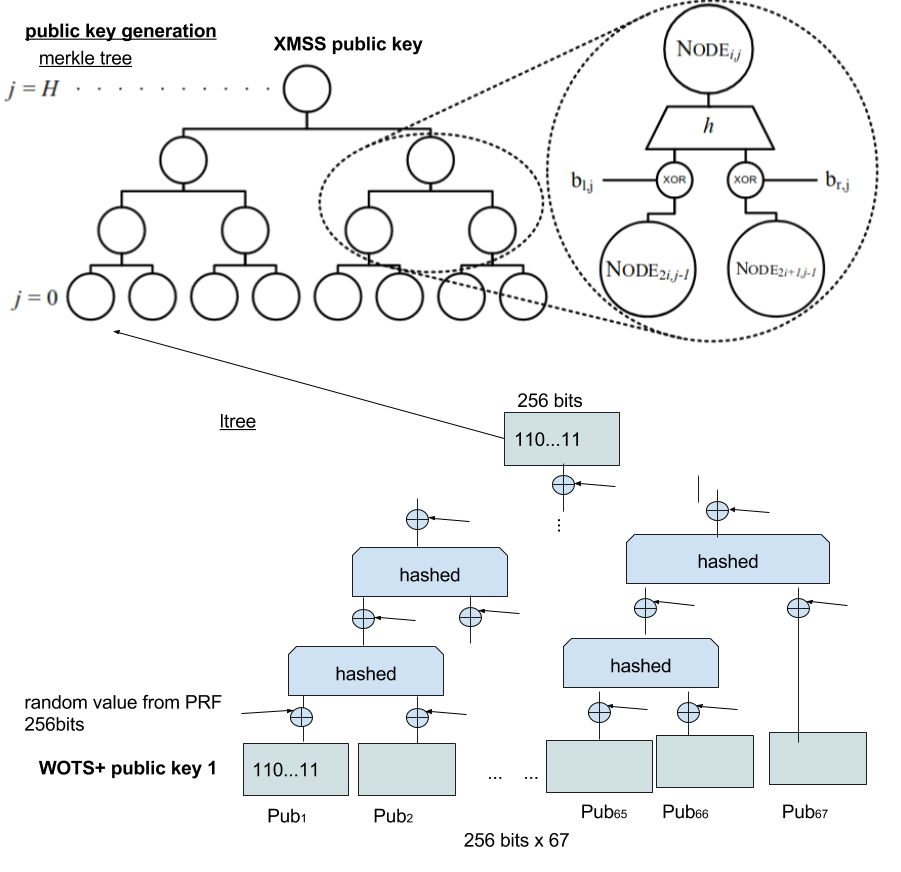
\includegraphics[width=80mm]{xmss_pub.png}
		  \caption{Key generation}
		\label{fig:xmss_pub}
		\end{center}
	 \end{figure}
	
	\vspace{-3.5mm}
	
	In short, XMSS builds a tree known as a `Merkle Tree',
	to gather all public keys into one single key. This then allows one public key to be reused many times.
	
	\vspace{2.5mm}
	
	Initially, one must generate \( 2^h \) WOTS+ private keys \( Priv_{ij}, i = 1 \ldots 2^h ,  j=1 \ldots 67\) and the
	corresponding WOTS+ public keys \( Pub_{ij}, i = 1 \ldots 2^h , j=1 \ldots 67 \)  (\(h\) is the height of Merkle Tree).
	Then, \(2^h\) number of `ltrees' are generated. \(i\)th (\(i = 1 \ldots 2^h\)) ltree is generated from
	\( Pub_{ij}, j = 1 \ldots 67 \). One receives the root hash of the \(i\)th
	ltree by hashing WOTS+ public keys (i.e. \( H(Pub_{i1} |  Pub_{i2} | \ldots  |  Pub_{i67} ) \)). The root hash of \(i\)th ltree
	becomes the \(i\)th leaf in the Merkle Tree. This operation is then repeated \( 2^h \) times to fill all remaining leaves of the Merkle Tree.
	Finally, the root hash of the Merkle Tree is calculated by hashing together the leaves of the Merkle Tree (i.e.\ roots of the ltrees). This root 
	hash becomes the XMSS public key.
	
	\vspace{2.5mm}
	
	When signing, one simply selects one of the unused private keys and its corresponding public key. Next, one calculates the WOTS+ signature. The 
	XMSS signature is the WOTS+ signature with an `auth path'. The auth path is an additional piece of binary data used to calculate the 
	root hash of the Merkle Tree (i.e.\ the XMSS public key).
	
	\newpage
	
	\begin{figure}[ht]
		\begin{center}
		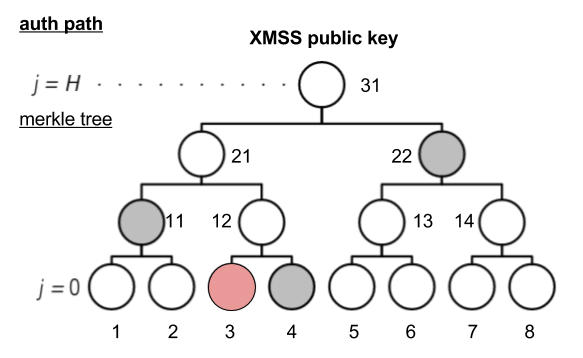
\includegraphics[width=80mm]{auth_path.png}
		  \caption{The auth path for XMSS}
		\label{fig:xmss_auth}
		\end{center}
	 \end{figure}
	
	\vspace{-3.5mm}
	
	With reference to Figure~\ref{fig:xmss_auth}, we desire to select private key \#3 for signing. A verifier can calculate node \#3 from the 
	signer's signature. However, in order to determine node \#12 the verifier will first need to determine node \#4, this means that the auth 
	path must include node \#4. In the same manner, in order to determine node \#31's root hash (i.e.\ the XMSS public key), the signer also 
	requires nodes \#11 and \#22 to be included within the auth path. Thus, in order to perform the verification, the verifier must posses the 
	WOTS+ signature and the node values along the auth path (i.e.\ the values of nodes \#4, \#11 and \#22). This will allow the verifier to 
	calculate the root hash of the Merkle Tree and determine if the root hash is equal to the XMSS public key.
	
	\vspace{2.5mm}
	
	Note that:
	\vspace{-0.5\baselineskip}
	\begin{itemize}
		\setlength\itemsep{0em}
		\item Signers must record which private keys are used. In order to accomplish this we use the Logarithmic Merkle Tree Traversal 
		scheme as presented in~\cite{traverse} to provide efficient traversal with minimal storage cost. \item The public key consists of 
		\(32 \times 2 \) bytes (the root hash of the Merkle Tree and the seed of the PRF). There is only one PRF seed, as all pseudo random 
		values can be generated from a single PRF\@. We include the seed as a part of the signature such that the public key size becomes 
		32 bytes. \item  The signature key size is approximately 3 kilobytes. \item The SHA-256 hash provides strong preimage resistance 
		(i.e.\ an attacker is unable to guess the input from the output of the hash), thus it is difficult to guess the private key from the public key, even when using quantum based hardware.
	\end{itemize}
			
	Additionally, note that we are able to reuse the same public key a number of times if \(h\) (the height of the Merkle Tree) is increased (although this requires more time to generate the public keys during the initial stage).
	
	\vspace{-2.5mm}
	
	\begin{table}[ht]
		\caption{Merkle Tree height, estimated time for key generation per CPU core, and intended users of XMSS}
		\label{tbl:height}
		\begin{tabular}{rrrl} 
			\toprule
			height  & \#keys & key generation & user \\ 
			\midrule
				  10 & 1,024 &  a few seconds & one time and\\
				  & & & normal users \\
				  16 & 65,536 & a few minutes & companies\\
				  20 & 1,048,576 & \( \approx \) 30 minutes &  big companies\\ 
				  \bottomrule
				\end{tabular}
	  \end{table}
	
	As Table~\ref{tbl:height} illustrates, there are 3 height levels for the Merkle Tree within Aidos Kuneen. Users who desire to change 
	addresses for each payment or who transact less than 1000 times with the same address are able to use height=10, reducing the impact of 
	generating public keys. Heavy users such as corporate entities or merchants, who transact more than 1000 times with one 
	public key, would use either height=16 or height=20.
	
	\vspace{2.5mm}
	
	Note: We have chosen not to use XMSS \(^{MT}\), as detailed in~\cite{ietf}. Although XMSS \(^{MT}\) means we do not need to generate all the public keys simultaneously, the signature size is much larger than that of XMSS, weighing in at around 40 kilobytes.
	
	\section{iMesh}
	\label{sec:imesh}
	
	\subsection{SPECTRE}
	When a sender sends a transaction, he includes some of the transactions previously sent by others. 
	Figure~\ref{fig:imesh} illustrates the DAG structure of these transactions which we refer to as \emph{iMesh}. When sending,
	the sender selects some of the leaves in iMesh (i.e.\ transactions which are not currently referred to by any other transactions) and 
	determines whether or not the parent transactions of these leaves are valid. After determining the parent transactions are valid the 
	leaves are included in the senders transaction.
	
	\begin{figure}[ht]
		\begin{center}
		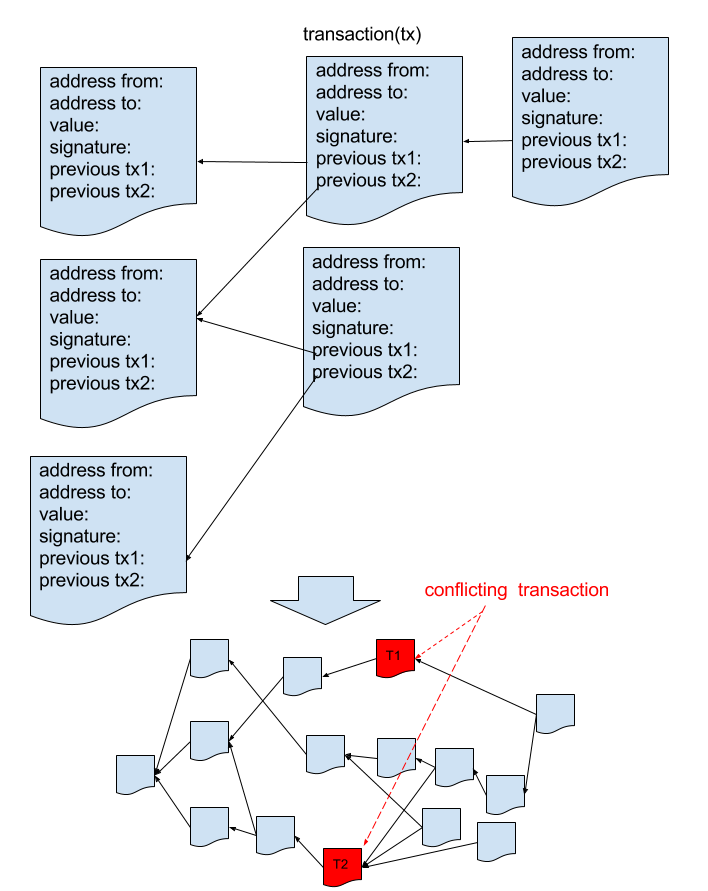
\includegraphics[width=65mm]{dag.png}
		  \caption{iMesh}
		\label{fig:imesh}
		\end{center}
	 \end{figure}
	
	\vspace{-3.5mm}
	
	Unlike block-chain based networks such as Bitcoin, where a block refers only to the preceding block, a single transaction in a DAG 
	refers to many other transactions within the DAG\@. With block-chain technology, the chain grows in a linear sequence (i.e.\ one block at a 
	time), whereas within a DAG the interlinked nature of the transactions allow it to grow simultaneously in all directions, thus leading 
	to superior scalability compared to block-chain based systems.
	
	\vspace{2.5mm}
	
	However, this interlinked nature is not without its drawbacks when it comes to conflicting transactions. For example, assume Alice's 
	address holds a total of 10 coins. She sends 10 coins to Bob in transaction T1, and then without thinking she sends 10 coins to Cathy 
	in another transaction T2. Alice has inadvertently attempted to spend the same coins twice (this is known as a `double spend')
	and as a result these two transactions are now in direct conflict. In a block-chain based system, once one of the conflicting 
	transactions has been written into a block, the other will be never stored, (i.e.\ if T1 receives at least one confirmation before T2, 
	then T2 will be rendered invalid). On the other hand when there are conflicting transactions (highlighted in red in 
	Figure\ref{fig:imesh}) within iMesh, it is difficult to determine which is valid. To solve this problem, Aidos Kuneen adopts the voting 
	mechanism as presented in `SPECTRE'~\cite{spectre}.
	
	
	\begin{figure}[ht]
		\begin{center}
		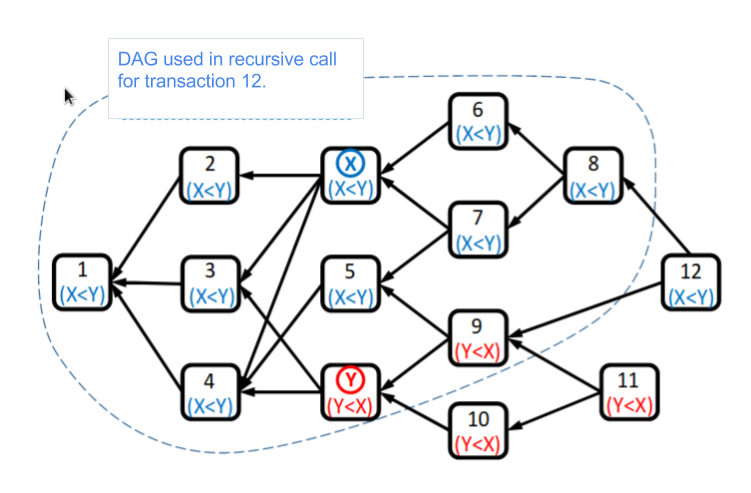
\includegraphics[width=80mm]{spectre.png}
		  \caption{An example of the voting procedure within a simplified DAG structure.}
		\label{fig:spectre}
		\end{center}
	 \end{figure}
	
	\vspace{-3.5mm}
	
	
	 In SPECTRE, one counts the number of voters for each of the conflicting transactions. Figure~\ref{fig:spectre} shows the voting 
	 procedure. As we can see, transactions X and Y are in conflict. Transaction X and transactions 6--8 vote for transaction X, as they 
	 only see X in their past, and not Y. Similarly, transaction Y and transactions 9--11 vote for transaction Y. Transaction 12 votes 
	 according to the majority of the votes from the other transactions (except for transactions 10, 11 and 12). All transactions from 1--5 
	 vote for transaction X as they see more X voters than Y voters. As a result, the total number of X voters is greater than Y voters, 
	 therefore X is accepted as the legitimate transaction and Y is rejected. 
	
	\vspace{2.5mm}
	
	 The rules regarding the SPECTRE voting procedure are summarised as follows:
	
	 \vspace{-0.5\baselineskip}
	 \begin{enumerate}
		 \setlength\itemsep{0em}
	\item Transactions which only have transaction X as the parent can only vote for transaction X. (transactions 6--8 and 9--11) 
	
	\vspace{1mm}
	Honest transactions gain votes over transactions that have been secretly withheld by dishonest parties, as honest nodes continue to add 
	new transactions that subsequently vote for the honest transaction.
	 \item Transactions which have both X and Y as a parent (transaction 12) vote for which ever one has the majority of voters. 
	
	\newpage
	
	This system guarantees majority amplification, as these transactions add votes that reinforce previous decisions. 
	 \item  Transactions which do not have both transactions X and Y as parents vote for which ever has the majority of voters (transaction 
	 1--5).
	
	\vspace{1mm}
	 This rule allows amplification of the votes of parents of transaction X (transaction 1--4). This is necessary to counter a `pre-mining 
	 attack' scheme, i.e.\ the attacker builds blocks and withholds them from the network. Due to the fact that honest transactions tend to 
	 have a greater number of ancestor transactions, an honest transaction should receive more votes by means of rules 1 and 2.
	 \end{enumerate}
	
	\vspace{-1.5mm}
	
	Note: SPECTRE is resilient against attackers with up to 50\% of the network's total computational power, and not the traditional 33\%, 
	as is demonstrated in~\cite{spectre}.
	
	\vspace{2.5mm}
	
	 Additionally, in iMesh receivers must also wait for their transaction to be confirmed by a sufficient number of other transactions 
	 (much like waiting for a number of `confirms' in Bitcoin) prior to spending. Reference~\cite{spectre} provides guidance on how long receivers 
	 should wait before trusting a new transaction. For comparison, let's assume that we will wait for 5 confirmations before accepting a 
	 payment on the Bitcoin network. Let's also assume that an attacker has managed to gain control of 30\% of the total hash power in the 
	 Bitcoin network. The possibility of success of such an attack is 17.8\%\cite{btc}. Similarly, in iMesh with the SPECTRE voting scheme 
	 employed, once a transaction (Tx A) has received approximately 130 referrals the probability of a fraudulent (intentionally conflicting) 
	 transaction (Tx B) being accepted as legitimate in place of Tx A has reduced to 17.8\%. As the iMesh network grows and the frequency of 
	 transactions increases, the waiting time required for a transaction to be verified as legitimate by the network will decrease (i.e.\ the 
	 larger the network grows the faster it becomes). Conversely, when the network is small, the waiting times are very long, the 
	 network hash power is also likely to be quite small and this is an opportunity that an attacker may attempt to exploit. 
	In order to prevent this potential attack vector, we introduce a mechanism known as `AKConsensus' (as discussed in Section~\ref{sec:AKConsensus}), 
	to confirm transactions between trusted full-nodes while iMesh is still in its infancy.
	
	\vspace{2.5mm}
	
	In the voting scheme, senders have an incentive to refer to as many transactions as they can due to the confirmation speed of the 
	sender's transaction being directly related to the number of referring transactions. If a sender were to refer to only a small number of 
	transactions, the receiver could potentially reject the payment as it would take a significant amount of time for the transaction to be 
	validated and for the receiver to receive the coins.
	
	\vspace{2.5mm}
	
	It must also be noted that if there are many leaves within iMesh, the possibility in which any one leaf is referred to by a new 
	transaction would reduce. To combat this we need to carefully consider how many transactions should be referred to by any one single 
	transaction. We will explore this issue in greater detail within Section~\ref{sec:leaves}.
	
	\subsection{AKConsensus}
	\label{sec:AKConsensus}
	
	As mentioned in the previous section, we must assume that during iMesh's infancy period an attacker with access to sufficient resources 
	could realistically command the majority of the total network hash power. It is for this reason that we are therefore unable to fully 
	trust the SPECTRE consensus mechanism during the early stages of network growth. Thus we must introduce `AKConsensus',
	a temporary system which utilises a Federated Byzantine Agreement (FBA) based on the `The Ripple Protocol Consensus Algorithm' 
	along with a semi-trusted model as detailed in~\cite{ripple}, in order to validate transactions until such time as the SPECTRE consensus mechanism can take over.
	
	\vspace{2.5mm}
	
	Within the Ripple Protoco,l the FBA process is used in order to confirm the validity of all transactions.
	A similar process, referred to as `AKConsensus' has been adopted for Aidos Kuneen, however, it should be noted that the implementation 
	of this process within Aidos Kuneen differs significantly from that of Ripple. 
	With AKConsensus in place, a group of trusted nodes periodically review a randomly selected transaction from within iMesh.
	If this group of trusted nodes reaches an agreement on the validity of this transaction, the transaction becomes known as a `Statement', and now serves to act as a milestone within the network.
	
	\vspace{2.5mm}
	
	The process of consensus is as follows:
	
	\vspace{-0.5\baselineskip}
	\begin{enumerate}
		\setlength\itemsep{0em}
		\item Each full-node defines the addresses of trusted nodes within their trusted list.
		\item One of the full-nodes selects a transaction for review and broadcasts it to the trusted nodes within their trusted list. 		This transaction is now referred to as a `Candidate Statement'.
		\item Each trusted node initialises \(T\) to 50\%.
		\item Each trusted node reviews the legitimacy of the Candidate Statement based on its local history.
		\item If a trusted node deems the Candidate Statement to be legitimate, it then broadcasts a `yes' vote to the full-nodes by which it is referenced. If the Candidate Statement is deemed to be fraudulent it is subsequently discarded.
		\item If a full-node does not receive a minimum of \(T\%\) of `yes' votes from the nodes on its trusted list within a certain period, the Candidate Statement is discarded.
		\item Each trusted node increases \(T=T+10\%\).
		\item Step 5.\ is repeated
		\item The final round requires a minimum of \(T=80\%\) of a full-node's trusted nodes in agreement in order to accept the the Candidate Statement as being legitimate and elevate it to the status of Statement.
	\end{enumerate}
	
	\vspace{1.5mm}
	
	Note: In order to be accepted as a Statement, a Candidate Statement must have a valid transaction structure and must exist within iMesh.
	
	\newpage
	
	 \begin{figure}[ht]
		\begin{center}
		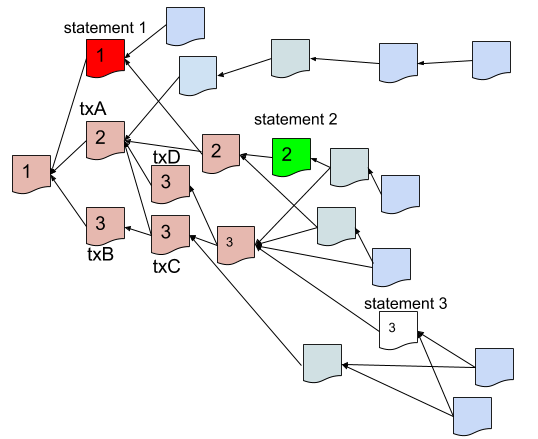
\includegraphics[width=80mm]{fba.png}
		  \caption{Statements and finalisation of transactions}
		\label{fig:fba}
		\end{center}
	 \end{figure}
	
	\vspace{-3.5mm}
	
	Figure~\ref{fig:fba} illustrates how Statements act as milestones for other transactions.
	Full-nodes regard Statements as an ``absolute truth'' and any conflicting transactions are discarded locally by each full node. 
	Subsequent transactions that are referred to by a Statement become known as Finalised Transactions.
	
	\vspace{2.5mm}
	
	The numbered transactions in Figure~\ref{fig:fba} show how transactions are finalised by the Statements that reference them,
	e.g.\ the transactions designated with \#2 are finalised by Statement \#2.
	
	\vspace{2.5mm}
	
	The rules employed by AKConsensus in order to determine the validity of conflicting transactions are as follows:
	
	\begin{itemize}
		\item The transaction which is finalised by the youngest Statement is deemed to be valid, and all others are considered to be invalid.
		\item If conflicting transactions are finalised by the same Statement, the transaction which possesses the older time stamp is deemed 
		to be valid.
		\item If both transactions possess the same time stamp, the transaction which has the smaller hash is deemed to be valid.
	\end{itemize}
	
	AKConsensus requires a minimum of 80\% agreement between trusted nodes in order to accept a Candidate Statement, and by extension, 
	20\% or more in order to reject an invalid Candidate Statement.
	
	\vspace{2.5mm}
	
	While it is acknowledged that the introduction of AKConsensus does directly contradict Aidos Kuneen's ultimate 
	vision of a completely decentralised cryptocurrency, AKConsensus, for the reasons outlined previously, is accepted to be a
	``necessary evil'' until such time as the network has matured to the point where it is capable of resisting attack on its own. 
	Additionally, Aidos Kuneen believes very strongly in providing a completely fee-less product to its user base,
	the presence of AKConsensus allows the realisation of this vision from day one, with no need to resort to alternative, `incentivised' 
	mechanisms for early network protection.
	
	\section{Proof of Work}
	\label{sec:PoW}
	
	When sending a transaction, senders must first perform `Proof of Work' (PoW), similar to that which is performed by miners in the 
	Bitcoin network. The mandatory performance of PoW prior to sending a transaction is necessary in order to protect iMesh from DDoS 
	attacks via spam transactions and double spend attacks (as previously discussed). In addition, PoW is used to distribute the 
	computational workload of validating transactions between all participants in the network. This ensures that the network does not 
	become constrained by the limitations in processing capabilities of a handful of `masternodes', but instead remains completely free to 
	scale as required. During the PoW operation each transaction is assigned a length \(L\), of 32-bit integer fields known as a `nonce'. 
	The value of this nonce is set such that the hash of the block will contain a leading run of zeros and form a series of `Cuckoo Graphs' with cycle length \(L\) (as is discussed in more detail below). The leading run of zeroes determines the time required for the PoW operation and has been chosen to produce an 
	average PoW time of 5--10 minutes.
	
	\vspace{2.5mm}
	
	For PoW operations, Aidos Kuneen implements the Cuckoo Cycle as discussed in~\cite{cuckoo}. The Cuckoo Cycle arises by the insertion of
	keys into a `Cuckoo Hashtable' which naturally leads to the cyclic formation of random bipartite graphs. A Cuckoo Hashtable consists of 
	two identical tables, each with a unique hash function which maps a key to a table location (this provides two possible locations for 
	each key). Upon arrival of a new key, its table location is first determined. If both possible locations are currently occupied by 
	existing keys, then one is extracted and inserted into its alternate location (potentially displacing yet another key). This process is 
	subsequently repeated until either a vacant location is identified, or a predetermined number of iterations is reached. This process 
	leads to the formation of cycles in what is referred to as a `Cuckoo Graph'. The Cuckoo Graph is a bipartite graph with a node at each 
	location, and an edge for every inserted key, connecting the two locations at which the key can reside.
	
	\begin{figure}[ht]
		\begin{center}
		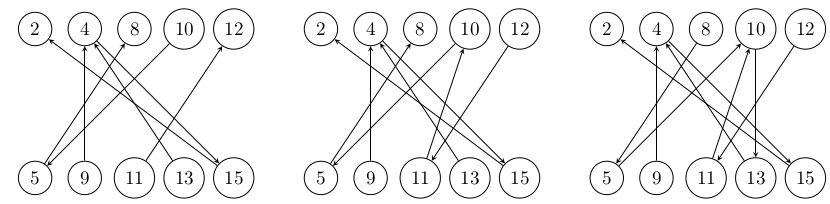
\includegraphics[width=80mm]{cuckoo.png}
		  \caption{Cuckoo Graph}
		\label{fig:cuckoo}
		\end{center}
	 \end{figure}
	
	\vspace{-3.5mm}
	
	The first diagram in Figure~\ref{fig:cuckoo} illustrates the directed Cuckoo Graph on \( N = 8 + 8 \) nodes after edges (2, 15), (4, 
	9), (8, 5), (4, 15), (12, 11), (10, 5) and (4, 13) are added. In order to add the 8th edge (10, 11), we follow the paths \( 10 
	\rightarrow 5 \rightarrow 8 \) and \( 11 \rightarrow 12 \) to find the different roots 8 and 12. Since the latter path is shorter, we 
	reverse the path to \( 12 \rightarrow 11\) such that we can add the new edge as (\( 11 \rightarrow 10\)), resulting in the middle 
	diagram. In order to add the 9th edge (10, 13) we now find the path from 10 to be the shorter one, so we reverse the path and add the 
	new edge as (\( 10 \rightarrow 13\)), resulting in the right diagram. When adding the 10th edge (8, 9), we find the paths
	 \( 8 \rightarrow 5 \rightarrow 10 \rightarrow 13 \rightarrow 4  \rightarrow 15 \rightarrow 2 \) and \( 9 \rightarrow 4 \rightarrow 15 
	 \rightarrow 2 \)  with equal roots. In this case, we can compute the length of the resulting cycle as 1 plus the sum of the path lengths to the node where the two paths join. In the diagram, the paths join at node 4, and the cycle length is computed as 1 + 4 + 1 
	 = 6.
	
	\vspace{2.5mm}
	
	The Cuckoo Cycle has been chosen as the PoW function for iMesh, due to the following reasons:
	
	\begin{itemize}
	\item We anticipate significantly higher daily transaction volumes compared to that of Bitcoin, this is due to the fact that unlike Bitcoin, the fee-less nature of Aidos Kuneen means the economic disincentive against frequently sending small transactions is removed. Thus, Aidos Kuneen requires a very fast verification method.
	
	
	\item Unlike other typical PoW algorithms such as Cryptonight or Scrypt which are typically quite resource intensive, full-nodes are able to verify the validity of nonces much faster when utilising the Cuckoo Cycle. 
	
	\item Unlike Bitcoin, in which PoW is performed only on the blocks themselves, in Aidos Kuneen PoW must be performed for each individual transaction. As there are significantly more individual transactions than there are blocks, Aidos Kuneen therefore requires more power to perform PoW verification. Thus, it is essential that a highly efficient means of verification, such as the Cuckoo Cycle is employed.
	
	\item In order to prevent an attacker from being able to propagate fraudulent transactions throughout the network, specialist hardware such as ASICs and FPGAs should not provide any advantage. As the PoW time is mainly dominated by memory access speed, specialist processing hardware is essentially rendered ineffective.
	\end{itemize}
	
	The following Cuckoo Cycle parameters will be used for PoW operations:
	
	\begin{itemize}
		\item cycle length \( L\) = 20 (To minimize the size impact on transactions).
		\item number of nodes \( N = 2^{25} \) (To provide memory usage of around 128MB\@).
		\item easiness \(N/M = 100\% , (M\): number of edges) (To prevent optimizations by edge trimming).
	\end{itemize}
	
	\section{Co-operative Proof of Work}
	\label{sec:coPoW}
	
	To cater specifically for IoT devices (whose performance is typically quite low), we introduce a novel co-operative Proof of Work 
	mechanism known as \emph{coPoW}. By utilising coPoW, the network is able to group a number of unverified transactions together into a 
	single, larger transaction known as a `Batch'. This allows the senders of the individual transactions within the Batch to effectively 
	pool their computational power into validating the Batch as a unit, rather than just their own individual transactions.
	coPow effectively acts like a decentralised version of a Bitcoin mining pool and allows large numbers of lower powered devices to interact directly with the network as if they were a single, much more powerful device.
	
	\vspace{2.5mm}
	
	coPoW functions as follows:
	
	\vspace{-0.5\baselineskip}
	\begin{enumerate}
		\setlength\itemsep{0em}
		\item A sender wishing to participate in coPoW broadcasts a request to network via a full-node.
		\item Others who wish to participate or are already performing coPoW respond to the request.
		\item The sender joins the coPoW group
		\item If the group is not yet established a process of leader selection is performed, if the group is already established then 
		the new device receives the identity of the existing leader.
		\item The sender sends his transaction to the leader who then mixes it with the transactions from all the other participants to 
		form a Batch.
		\item All senders commence PoW on the Batch.
		\item The sender periodically sends the result of their `PoW for proof' (which meets the requirement for the `target for proof') to the leader.
		\item The sender periodically receives the PoW results from other parties via the leader. 
		\item If any of the parties submit incorrect results they are ejected from the group.
		\item If any of the parties fail to submit their results within a set period of time, the leader ejects that party and then 
		delivers a restart command to all remaining parties.
		\item The process continues until one of the parties successfully solves for the `final hash', after which PoW is completed and 
		the group is disbanded.
	\end{enumerate}
	
	Parties participating in a coPoW group must periodically send some of their PoW results to the leader to prove 
	that they are actively participating in the group. This prevents free-loading by parties who join the group but do not intend to 
	actively contribute. The \emph{target for proof} threshold is set such that the hash is less complex than the \emph{final hash},
	this is important to ensure that devices with limited computational capacity are able to successfully meet the 
	target for proof within the required time period. The target for proof itself can be variable. For example, target for proof = final 
	target \(  \times 2^{-5} \) could be adopted for groups of low capacity IoT devices, and the target for proof = final target  \( \times 
	2^{-2} \) could adopted for normal desktop PCs.
	
	\vspace{2.5mm}
	
	For added anonymity, participants in a coPoW group have the option to utilise the Tor network for all communications between themselves 
	and the group. 
	
	\section{AKShuffle}
	\label{sec:aks}
	
	For increased anonymity we employ \emph{AKShuffle}. Within AKShuffle we utilize a zero-knowledge, non-interactive (ZKNI) proof for
	anonymous transactions. By utilising ZKNI, one can prove that their value satisfies a set of functions without the need to reveal their 
	secret key. For example: Alice has input \(x\) and key \( k \) for an encryption function \( f_{k}(x) \), and shares \( y=f_k(x) \) 
	with Bob. Bob wants to know if Alice really has key \(k\), but Alice doesn't want to reveal her secret key to Bob. By employing ZKNI, 
	Alice can prove to Bob that she really has key \( k\) without ever actually having to reveal the key itself.
	
	\vspace{2.5mm}
	
	Aidos Kuneen utilizes `ZKBoo (ZKB++)' as presented in~\cite{zkb} as its ZKNI mechanism. ZKBoo requires only the use of a hash and an 
	AES encryption function which has been shown to be quantum secure~\cite{pqcrypto}.
	
	\begin{figure}[ht]
		\begin{center}
		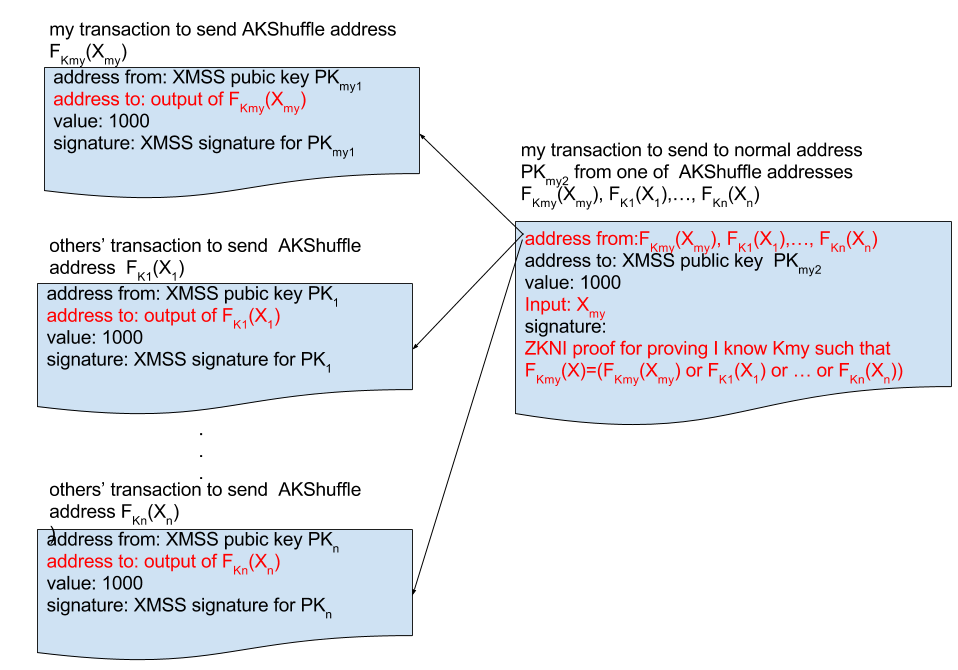
\includegraphics[width=80mm]{shuffle.png}
		  \caption{An example of how AKShuffle operates}
		\label{fig:shuffle}
		\end{center}
	 \end{figure}
	
	\vspace{-3.5mm}
	
	With reference to Figure~\ref{fig:shuffle}, the operation of AKShuffle is described as follows:
	\vspace{2.5mm}
	
	Any user who desires to shuffle their tokens simply sends them to an AKShuffle address.
	The shuffle address is an output of the encryption \( f_{k_{my}}(x_{my}) \) with key \( k_{my} \),  
	where \(k_{my}\) is the secret key  and \(x_{my}\) is the public input.
	If at any point the user desires to withdraw their shuffled tokens they simply create a transaction which sends the tokens to their 
	normal address \(PK_{my_2}\) (i.e.\ their XMSS public key).
	The transaction contains the user's AKShuffle address \( f_{k_{my}}(x_{my}) \) along with other user's AKShuffle addresses 
	\( f_{k_{1}}(x_{1}) \), \( f_{k_{2}}(x_{2}) \) \dots \( f_{k_{n}}(x_{n}) \) as input addresses. 
	This means that nobody knows which address has actually been used for the withdrawal. 
	In order to prove ownership the user completes the ZKNI proof by proving they know \( k_{my} \) such that one of the AKShuffle 
	addresses listed as an input equals \( f_{k_{my}}(x_{my}) \). 
	The transaction also includes the user's public input \( x_{my} \) in order to prevent to the reuse of the shuffle address. It is also 
	important to point out that the user is required to withdraw the full amount that they originally deposited, 
	the system will not allow partial withdrawals of the user's balance as reuse of a shuffle address is strictly forbidden in order to maintain anonymity.
	
	\vspace{2.5mm}
	
	Note: Transactions used for AKShuffle and transactions user for normal payments are completely different. AKShuffle (ZKBoo) is used 
	only for shuffling one's tokens. As such, one cannot use AKShuffle to send tokens directly to another user. This is due to the fact 
	that the signature size of ZKBoo is quite large, weighing in at around 500 kilobytes for 5 inputs.
	
	\newpage
	
	\section{Network}
	\label{sec:network}
	
	\begin{figure}[ht]
		\begin{center}
		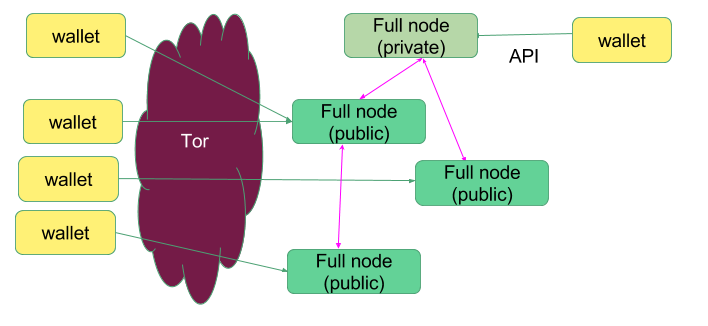
\includegraphics[width=80mm]{network.png}
		  \caption{Aidos Kuneen network topology}
		\label{fig:network}
		\end{center}
	 \end{figure}
	
	\vspace{-3.5mm}
	
	
	As illustrated in Figure~\ref{fig:network}, the Aidos Kuneen network is comprised of a series of full-nodes who communicate in a P2P fashion. 
	Clients can either connect directly to these full-nodes or to their own full-node via API\@. Clients are able to send API requests in order to broadcast their transactions to the network (this is usually performed automatically
	by the wallet application). Between full-nodes, transactions are sent and received using an efficient serialization (e.g.\ msgpack\footnote{https://msgpack.org/}) in order to reduce packet sizes.
	
	\vspace{2.5mm}
	
	In order to ensure anonymity between public full-nodes and clients we utilise the Tor network. This is essential as full-nodes
	may otherwise receive sensitive information such as their clients' IP addresses along with the clients' transactions.  
	
	\vspace{2.5mm}
	
	It is important to note that Tor is not employed for communications between full-nodes. This is due to the fact that routing traffic via the Tor network introduces an unavoidable element of delay into inter-nodal communications, and efficiency between full-nodes 
	is a critical aspect of the speed of the entire Aidos Kuneen network. Additionally, there is little need to enforce anonymous communication between nodes, this is due to the fact that even if the initial client-to-node connection were not secured with Tor, the initial receiving node 
	does not transmit any sensitive information about the client when it relays the transaction to the other nodes.
	
	\vspace{2.5mm}
	
	Unfortunately however, Tor is not quantum secure. Though, Tor does have the advantage of being a well established, trusted network with a large number of participants. We believe that for the short term at least, the strong anonymity provided 
	by the Tor network is an excellent fit for Aidos Kuneen. We will continue to investigate other potential methods of providing quantum-resistant anonymity as they become available. 
	
	\vspace{2.5mm}
	
	Table~\ref{tbl:cmd} lists the basic packet commands for the Aidos Kuneen network.
	
	\newpage
	
	%\clearpage
	
	 \begin{table}[htb]
		\caption{Basic Packet Commands}
		\label{tbl:cmd}
		\begin{tabularx}{\linewidth}{XX} 
			command & description \\
			\toprule
	  ping & ping to another node \\
	  pong & response of ping \\
	  find\_node & request node info\\
		resp\_node & response node infers \\
	  req\_transactions & request transactions contents \\
	  resp\_transactions & respond transactions contents \\
	  req\_leaves & request  leaves' hashes \\
	  resp\_leaves &  respond leaves' hashes \\
	  invent &  invent new transaction hash \\
	  ack\_invent & ack of invent \\
	  invent\_copow & invent that a node is searching for coPoW group \\
	  ack\_copow & ack of invent\_coPoW \\
	  find\_value &  reserved for future use.\\
	  store\_value & reserved for future use.\\
	  \bottomrule
	\end{tabularx}
	  \end{table}
	
	\section{Leaves within iMesh}
	\label{sec:leaves}
	
	As mentioned previously in Section~\ref{sec:imesh}, the speed of confirmation
	depends heavily on the number of leaves, \( N_{leaves} \), in iMesh. This is due to the fact that as the number of leaves within iMesh increases,
	the probability that a new transaction will refer to any one leaf reduces. 
	
	\vspace{2.5mm}
	
	There are a number of scenarios in which the number of leaves could conceivably increase, as illustrated in Figure~\ref{fig:leaves}:
	
	\begin{figure}[ht]
		\begin{center}
		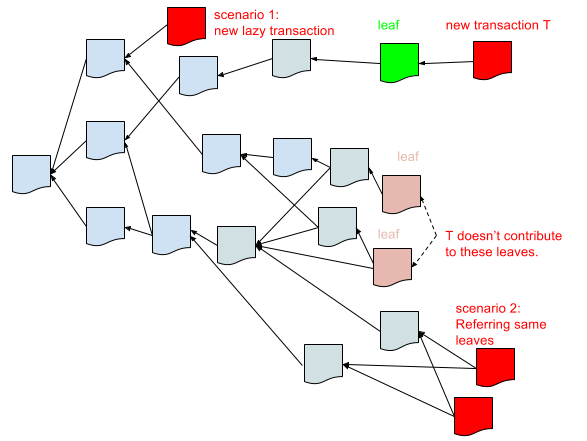
\includegraphics[width=80mm]{leaves.png}
		  \caption{Leaves within iMesh}
		\label{fig:leaves}
		\end{center}
	 \end{figure}
	
	\vspace{-3.5mm}
	
	The first scenario is that an attacker might seek to slow down iMesh by intentionally referring to non-leaf transactions.
	This would have the effect of adding additional, unreferenced leaves to the DAG, thus decreasing the overall efficiency of the entire network.
	
	\vspace{2.5mm}
	
	In order to combat this situation we could set \( N_{ref} \geq 3 \) to help prevent attackers from increasing the number of leaves indiscriminately.
	If we combine this with the fact that an attacker can only add one new leaf per transaction, we will find that (provided the attacker does not control more than 50\% of the total network hash power) honest transactions will rapidly 
	reference the attacker's new leaves, thus integrating them into the DAG and preventing the uncontrolled growth of unreferenced leaves.
	
	\vspace{2.5mm}
	
	In a similar situation to scenario one, an attacker may seek to spam the network by broadcasting a large number of very low (or even zero value) transactions to either himself or an accomplice in an attempt create a large number of leaves in a short 
	amount of time, thus causing confirmation times to significantly increase. This is easily prevented by the existing requirement to complete PoW for every transaction, regardless of the value being transacted.
	
	\vspace{2.5mm}
	
	In the third scenario, one transaction \(T_1\) could enter into iMesh while another, \(T_2\), is still in the process of being validated (i.e.\ still undergoing PoW) and has not yet appeared in iMesh.
	Thus \(T_1\) and \(T_2\) may actually both be referring to the same reference transaction.
	This scenario is not necessarily the result of malicious intent, in fact, it could be expected to occur quite frequently during normal network operation.
	
	\vspace{2.5mm}
	
	To solve this problem, we could increase the number of referring transactions for any one transaction, \( N_{ref} \), in order 
	to decrease \( N _{leaves} \) (i.e.\ to converge iMesh). However, this has the undesirable side effect of increasing the transaction size.
	As such, we need to determine the optimal \( N_{ref} \) value in order to converge iMesh, while still seeking to maintain a small transaction size. 
	
	\vspace{2.5mm}
	
	To this end, we will now present a simulation of the behavior of iMesh.
	
	\vspace{2.5mm}
	
	Firstly, we assume the process of incoming transactions can be modelled by a Poisson flow, the size of a  transaction  \(|Tx|\)  is given by (\( \text{constant} + 32 \times N_{ref}\)) bytes, and the time to complete PoW can be modelled by an exponential distribution.
	So, let \(\lambda_{in}\) equal the rate of the Poisson flow  and \(1 / \lambda_{pow}\) equal the expected time to complete PoW.
	Therefore, we can say that on average, users will produce transactions at rate of \(\lambda_{in}\) and will complete PoW in \(1/\lambda_{pow}\).
	Note: The transaction rate includes PoW time \(1/\lambda_{pow}\).
	
	\vspace{2.5mm}
	
	While a user is performing PoW, other users will be generating new transactions and these transactions will likely include some of the same reference transactions as the transaction currently undergoing PoW.
	The fact that \( N_{ref} (t) \) depends on \( N_{ref} (t-t')\) (i.e.\ the status in the past) makes it difficult 
	to solve for \( N_{ref}\) directly. Hence, it becomes necessary to simulate the behaviour of \( N_{ref}\).
	
	\vspace{2.5mm}
	
	Algorithm~\ref{alg:sim1} shows the algorithm used to simulate the number of leaves in iMesh.
	We take \(1 / \lambda_{pow} = 10 \) minutes and simulate with \(N_{ref}\ = 2, 4, 8, 16, 32 \) across the following rates of input transactions \(\lambda_{in} \):
	
	\vspace{-0.3\baselineskip}
	\begin{enumerate}
		\setlength\itemsep{0em}
	\item \(\lambda_{in} \)=1 transaction per minute 
	 (This models the early days of iMesh when the user base is small)
	\item \(\lambda_{in} \)=1 TPS (transaction per second)
	\item \(\lambda_{in} \)=5 TPS 
	 (This is the peak transaction speed in the Bitcoin network as occurred in May 2017)
	 \item \(\lambda_{in} \)=10 TPS
	\end{enumerate}
	
	\vspace{-3.5mm}
	
		\begin{algorithm}[ht]                  
			\caption{Simulation of the number of leaves within iMesh}         
			\label{alg:sim1}
			\begin{algorithmic}\fontsize{10pt}{10pt}\selectfont
				\STATE{INPUT  \(N_{ref}\): number of directly referring transactions}
				\STATE{INPUT \(T_{sim}\): number of iterations}
				\STATE{INPUT \(\lambda_{in}\): rate of incoming transactions}
				\STATE{INPUT \(\lambda_{pow}\): time to complete PoW }
				\STATE{OUTPUT\@: number of leaves}
				\STATE{}
		\STATE{\(time=0\) //current time}
		\STATE{\(pow\_txs=\{\} \) //transactions which are undergoing PoW}
		\STATE{\(txs=\{\} \) //transactions in iMesh}
		\WHILE{\(time < T_{sim}\)}
			\STATE{\(step \Leftarrow \) an exponentially distributed value at rate \(\lambda_{in}\)}
			\STATE{\(time \Leftarrow time + step\)}
		
			\STATE{}
		\STATE{//add a new transaction to the transaction list}
		\STATE{//with a period to complete PoW.}
		\STATE{make new transaction \(t_{new}\)}
		\STATE{\(t_{new}.is\_leaf \Leftarrow true\)}
		\STATE{\(leaves \Leftarrow \) select random \(N_{ref}\) leaves in \(txs\)}
		\STATE{\(t_{new}.leaves \Leftarrow leaves\)}
		\STATE{\(pow\_time \Leftarrow \) an exponentially distributed value at rate \(\lambda_{pow}\)}
		\STATE{\(t_{new}.pow\_time \Leftarrow time + pow\_time\)}
		\STATE{append \(t_{new}\) to \(pow\_txs\)}
		
		\STATE{}
		\STATE{//handle transactions whose PoW has finished}
		\FORALL{\(t\) in \(pow\_txs\)}
		\IF{\(t.pow\_time \le time\)}
		\STATE{remove \(t\) from \(pow\_txs\)}
		\STATE{append \(t\) to \(txs\)}
		\FORALL{\(l\) in \(t.leaves\)}
		\STATE{\(l.is\_leaf \Leftarrow false\)}
		\ENDFOR{}
		\ENDIF{}
		\ENDFOR{}
		\STATE{count \(t\) such that \(t.is\_leaf=true\) in \(txs\) and print it}
		\ENDWHILE{}
		\end{algorithmic}
			\end{algorithm}
	
	\vspace{-3.5mm}
	
	Figures~\ref{fig:min1_2} \textasciitilde~\ref{fig:sec10} in Appendix A show the results of the simulation.
		 The result of \( N_{ref}=8,16,32\) for \( \lambda_{in}=1\) transactions per minute are not included
		 as these results essentially the same as those of \( N_{ref}=4\).
	
	\vspace{2.5mm}
	
		 From these results, we can see that the number of leaves \( N_{leaves}\) decreases in proportion to the increasing value of \( N_{ref} \).
		 Even when \( \lambda_{in}=1\) transaction per minute, \( N_{ref}=2\) is not enough to fully converge the DAG, (\( N_{leaves}\) is around 3 \textasciitilde~26),
		 and \( N_{ref} \ge 4\)  is better (\( N_{leaves}\) = 1 \textasciitilde~18).
		 Furthermore, when we look at the other \( \lambda_{in}\) values, we notice that \( N_{ref}=2\) is considerably worse than the other \( N_{ref}\) values.
		 For example, at \( \lambda_{in}=5\) TPS,  \( N_{leaves} \simeq 3800 \) when \( N_{ref}=2\),
		\( N_{leaves} \simeq 500\)  when \( N_{ref}=8\). Therefore, it is clear that we should \emph{NOT} use \( N_{ref}=2\) if we assume 
		transactions enter into iMesh at same speed as Bitcoin.
		The time to converge DAG is below 3000 seconds (50 minutes) for all values of \( N_{ref} \) except \( N_{ref}=2\) when \( \lambda_{in}=10\) TPS\@.
	
	\vspace{2.5mm}
		
		It should also be mentioned that as \(|Tx|\) exhibits simple linear behaviour and doubles with each increase in the value of \( N_{ref} \), from a purely transaction size focused point of view, we should seek 
		to minimise the \( N_{ref} \) value.
	
	\vspace{2.5mm}
		
		We also simulate how the number of transactions, \( N_{descendant} \), which refer directly and indirectly to any one transaction grow 
		 for each of the cases mentioned previously. Figures~\ref{fig:min1_ref} \textasciitilde~\ref{fig:sec10_ref} in Appendix B illustrate these results.
	
	\vspace{2.5mm}
		 
		 In these figures, the x-axis shows the number of transactions which enter into iMesh (after iMesh has become stable). The y-axis shows \( N_{descendant} \) 
		 (the number of descendant transactions) for one random transaction. The graph would become a diagonal (linear) line if \( N_{descendant} \) were to grow at an ideal rate.
		 When \( \lambda_{in}=\) 1 transaction per minute, the graphs of all \( N_{ref}\) are almost diagonal.
		 But, as \( \lambda_{in}\) increases,  \( N_{descendant} \) reduces.
		 For example, when \( \lambda_{in}\) =5 TPS, \( N_{descendant} \) 
		 does not increase diagonally even after  25000 transactions (\( 25000 \times 0.2\) seconds \(\simeq 1.39 \) hours on average) at \( N_{ref} \) = 2.
	When \( N_{ref}\)= 8 and after 4000 transactions (\( 4000 \times 0.2\) seconds \(\simeq 13.3 \) minutes on average),
	 \( N_{descendant}\) starts to increase linearly.
	
	\vspace{2.5mm}
	
		 As such, we believe that the best course of action is to allow \( N_{ref}\) to remain as a variable. \( N_{ref}=8\) will be adopted at the initial setting, due to the fact that 
		 even if iMesh were to grow to \( \lambda_{in}=5\) TPS (which is the maximum TPS
		 in Bitcoin), \( N_{ref}=8\) still allows iMesh converge at around \#leaves=500. 
		 Additionally, as previously discussed, setting \( N_{ref}=8 \geq 3\) will
		 help to prevent attackers from increasing the number of leaves indiscriminately.
	
	\vspace{2.5mm}
		
		  As iMesh continues to grow we will review the value of the \( N_{ref}\) variable in order to maintain optimal network performance.
		  
	\section{Future Plans}
	\label{sec:future plans}
	
		The following plans are intended to be integrated into the Aidos Kuneen network in the future:
		 
	
		\vspace{-0.5\baselineskip}
		\begin{enumerate}
			\setlength\itemsep{0em}
		\item  Distribute transactions between nodes to allow for increased scalability (i.e.\ a single full-node does not hold all transactions 
		 within the network but instead queries other nodes in the network as required)
		\item Implement a Kademlia based scheme for Tor-like anonymity, post-quantum security and distributed peer discovery.
		\item Implement a more sophisticated ZKNI algorithm in order to reduce transaction sizes.
		\end{enumerate}
	
		  \section{Conclusion}
	\label{sec:conc}
	
	In this white paper we have presented the new cryptocurrency \emph{Aidos Kuneen}.
	
	\vspace{2.5mm}
	
	Aidos Kuneen employs \emph{iMesh}, where all transactions are directly referred to one another in order to form a DAG structure.
	
	\vspace{2.5mm}
	
	To prevent double spending we utilize `SPECTRE' to determine the legitimacy of all transactions.
	
	\vspace{2.5mm}
	
	We employ the hash-based signature `XMSS' as the signature scheme for post-quantum resistance.
	
	\vspace{2.5mm}
	For anonymity we introduce \emph{AKShuffle} which utilises the zero-knowledge proof `ZKBoo (ZKB++)' for post-quantum security.
	
	\vspace{2.5mm}
	
	To cater for the future growth of the IoT sector we introduce a novel cooperative Proof of Work mechanism called \emph{coPoW}, which allows low powered devices to combined their resources and perform PoW as a group.
	
	\vspace{2.5mm}
	
	Finally, we provided a simulation of the number of leaves within iMesh, and the expected behaviour of the network as the network grows.
	
	\vspace{3cm}
	\begin{table}[htb]
		\caption{Aidos Kuneen: Technical Specifications}
		\label{tbl:spec}
		\begin{tabularx}{\linewidth}{XX} 
			\toprule
			Ticker & ADK \\
			\midrule
	Total Supply & 25,000,000 ADK \\ 
	\midrule
	Minimum Unit & 0.00000001 (\(10^{-8})\) ADK \\ 
	\midrule
	PoW Algorithm & Cuckoo Cycle\\ 
	\midrule
	Anonymity & AKShuffle (post-quantum zero knowledge proof) and Tor \\
	\midrule
	Consensus Algorithm & SPECTRE \\ \midrule
	Distributed Ledger & iMesh (transaction DAG) \\
	\midrule
	Signature Scheme & XMSS (post quantum hash based signature)\\ 
	\midrule
	Usage &  Finance, Banking, Digital Commerce, IoT Micropayments \\ 
	\bottomrule
	\end{tabularx}
	  \end{table}
	
	\vspace{3cm}
	
	\begin{center}
	
\includegraphics[width=40mm]{logo-min}\\[\bigskipamount]
	\end{center}
	
	  \twocolumn[
		\begin{@twocolumnfalse}
	
	
	  \begin{thebibliography}{99}
		
		\bibitem{btc}
			Satoshi Nakamoto,
			\emph{Bitcoin: A Peer-to-Peer Electronic Cash System}, 2008.
		
		\bibitem{ietf}
		Crypto Forum Research Group, draft-irtf-cfrg-xmss-hash-based-signatures-10
			\emph{XMSS:Extended Hash-Based Signatures}, 2017.
			
		\bibitem{iota}
		Serguei Popov,
			\emph{The tangle}, 2017.
		
		\bibitem{prob}
		Sheldon M. Ross,
			\emph{Introduction to Probability Models. 10th Edition}, 2012.
		
		\bibitem{dagcoin}
		Sergio Demian Lerner,
			\emph{DagCoin: a cryptocurrency without blocks}, 2015.
		
		\bibitem{xmss}
		Johannes Buchmann, Erik Dahmen, Andreas H\"ulsing,
			\emph{XMSS --- A Practical Forward Secure Signature Scheme Based on Minimal Security Assumptions}, 2011.
		
		\bibitem{zkboo}
		Irene Giacomelli, Jesper Madsen, Claudio Orland,
			\emph{ZKBoo: Faster Zero-Knowledge for Boolean Circuits}, 2016.
			
		\bibitem{zkb}
		Melissa Chase, David Derler, Steven Goldfeder, Claudio Orlandi, Sebastian Ramacher, Christian Rechberger, Daniel Slamanig, Greg Zaverucha,
			\emph{Post-Quantum Zero-Knowledge and Signatures from Symmetric-Key Primitives}, 2017.
			
		\bibitem{spectre}
		Yonatan Sompolinsky, Yoad Lewenberg, and Aviv Zohar, 
			\emph{SPECTRE\@:	Serialization of Proof-of-work Events: Confirming Transactions via Recursive Elections}, 2016.
		
		\bibitem{shor}
		Peter W. Shor, 
			\emph{Polynomial-Time Algorithms for Prime Factorization and Discrete Logarithms on a Quantum Computer}, 1995.
			
		\bibitem{google}
		Masoud Mohseni, Peter Read, Hartmut Neven,
			\emph{Commercialize early quantum technologies}, 2017.
			
		\bibitem{recom}
		PQCRYPTO,
			\emph{Post-Quantum Cryptography for Long-Term Security, Initial recommendations of long-term secure post-quantum
			systems}, 2015.
				
		\bibitem{ringsig}
		Nicolas van Saberhagen,
			\emph{CryptoNote v 2.0}, 2013.
	
		\bibitem{cuckoo}
		John Tromp,
			\emph{Cuckoo Cycle: a memory bound graph-theoretic proof-of-work}, 2014.
	
		\bibitem{byteball}
		Anton Churyumov,
			\emph{Byteball: A Decentralized System for Storage and 	Transfer of Value}.	
	
		\bibitem{traverse}
		Michael Szydlo,
			\emph{Merkle Tree Traversal in Log Space and Time}, 2004.	
	
		\bibitem{pqcrypto}
			PQCRYPTO,
				\emph{Post-Quantum Cryptography for Long-Term Security}, 2015.	
		
		\bibitem{ripple}
		David Schwartz, Noah Youngs, Arthur Britto,
				\emph{The Ripple Protocol Consensus Algorithm}, 2014.	
		
	
		\end{thebibliography}
		
		\end{@twocolumnfalse}
		]
	
	
	\clearpage
	
	\begin{appendices}
		\twocolumn[
		\section{Results of Simulation --- Number of Leaves ) }
		]
	\label{Appendix A}
	
	\begin{figure}[H]
		\begin{center}
		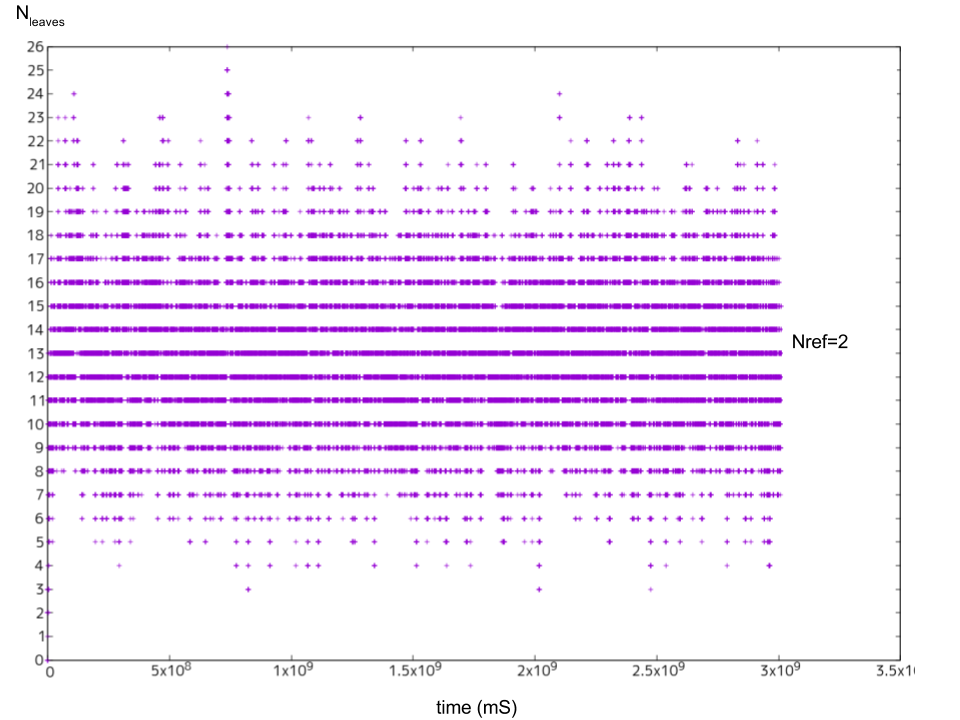
\includegraphics[width=80mm]{1min_2.png}
		  \caption{\( \lambda_{in}=\) 1 transaction per minute, \( N_{ref}=2\)}
		\label{fig:min1_2}
		\end{center}
	 \end{figure}
	
	 \begin{figure}[H]
		\begin{center}
			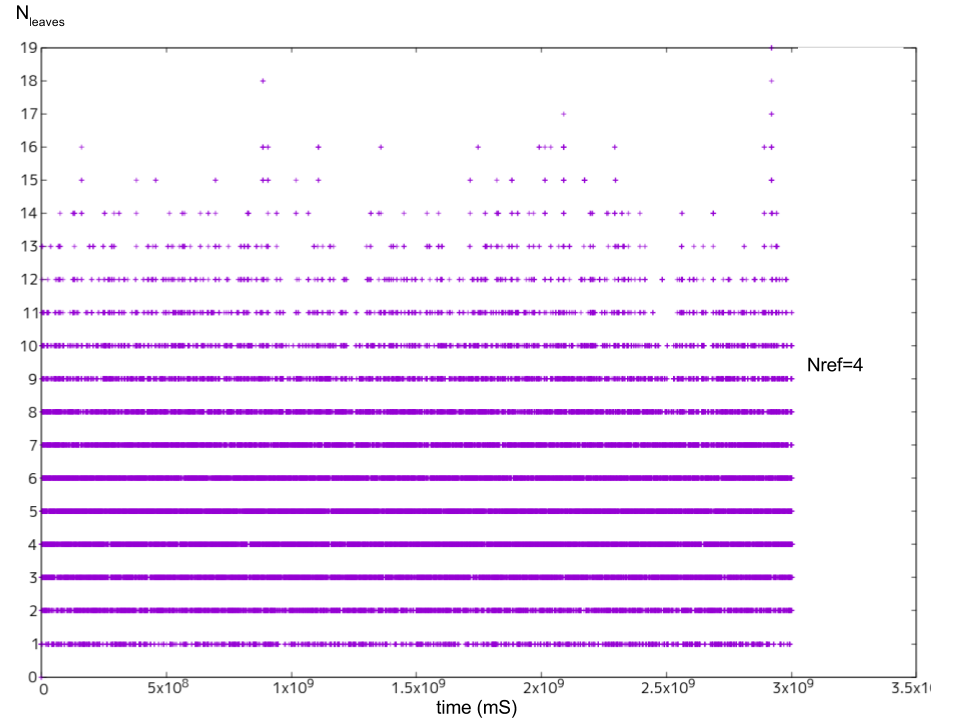
\includegraphics[width=80mm]{1min_4.png}
			\caption{\( \lambda_{in}=\) 1 transaction per minute, \( N_{ref}=4\)}
		  \label{fig:min1_4}
		\end{center}
	 \end{figure}
	
	 \begin{figure}[H]
		\begin{center}
		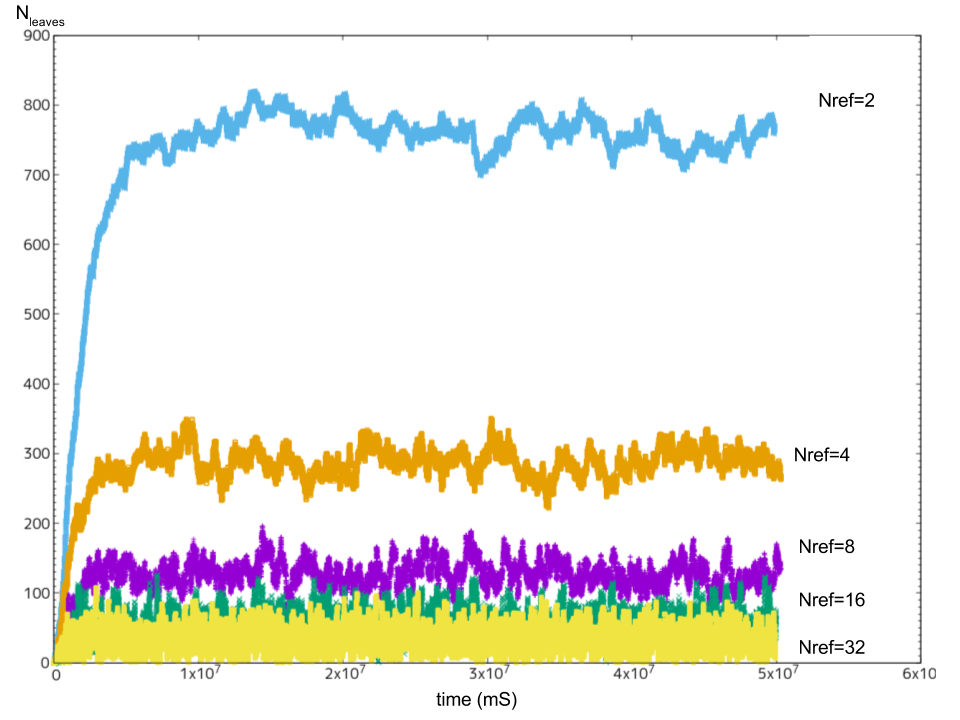
\includegraphics[width=80mm]{1sec.png}
		  \caption{\( \lambda_{in}=\) 1 TPS}
		\label{fig:sec1}
		\end{center}
	 \end{figure}
	
	 \space{1cm}
	
	 \begin{figure}[H]
		\begin{center}
		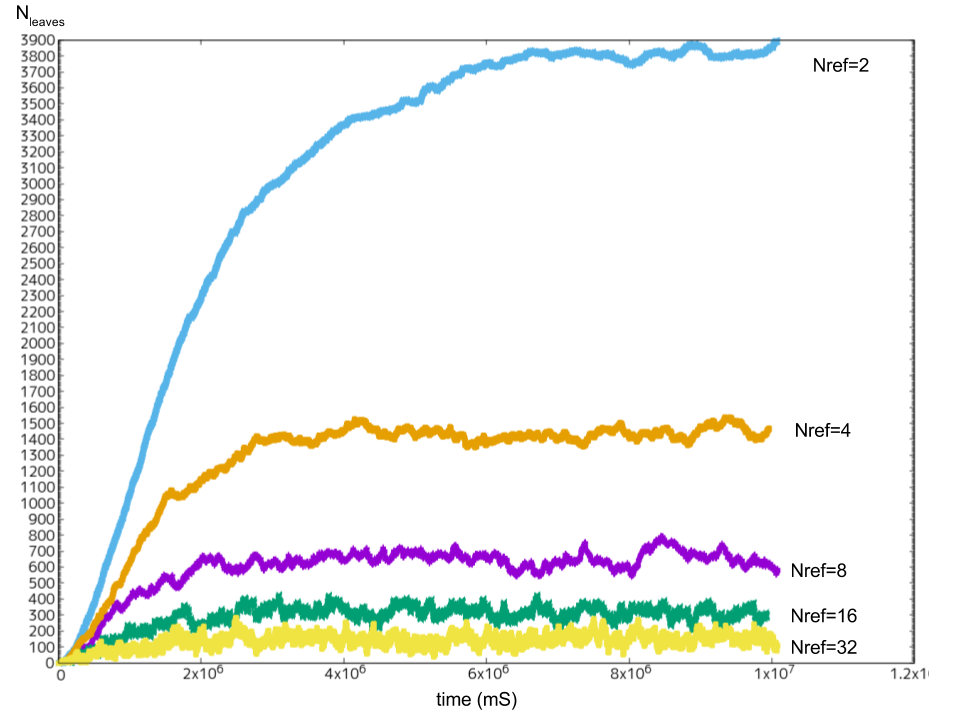
\includegraphics[width=80mm]{5sec.png}
		  \caption{\( \lambda_{in}=\) 5 TPS}
		\label{fig:sec5}
		\end{center}
	 \end{figure}
	
	 \begin{figure}[H]
		\begin{center}
		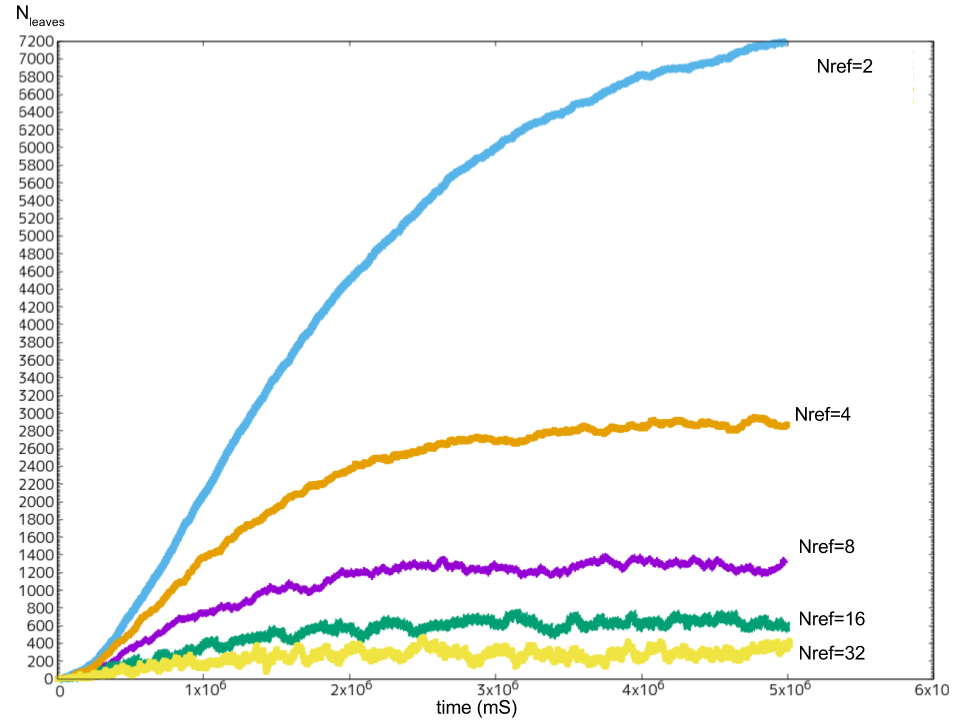
\includegraphics[width=80mm]{10sec.png}
		  \caption{\( \lambda_{in}=\) 10 TPS}
		\label{fig:sec10}
		\end{center}
	 \end{figure}
	\end{appendices}
	
	 \begin{appendices}
		\twocolumn[
		\section{Results of Simulation --- Growth of}
		]
	\label{Appendix B}
	
	 \begin{figure}[H]
		\begin{center}
			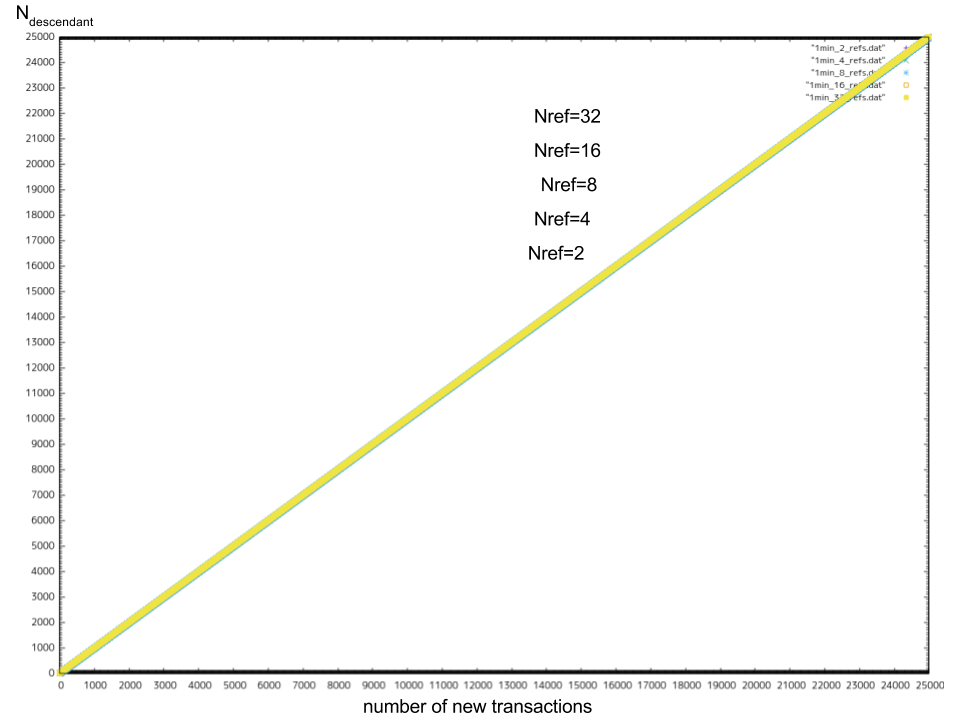
\includegraphics[width=80mm]{1min_ref.png}
			\caption{\( \lambda_{in}=\) 1 transaction per minute}
		  \label{fig:min1_ref}
		\end{center}
	 \end{figure}
	
	 \begin{figure}[H]
		\begin{center}
			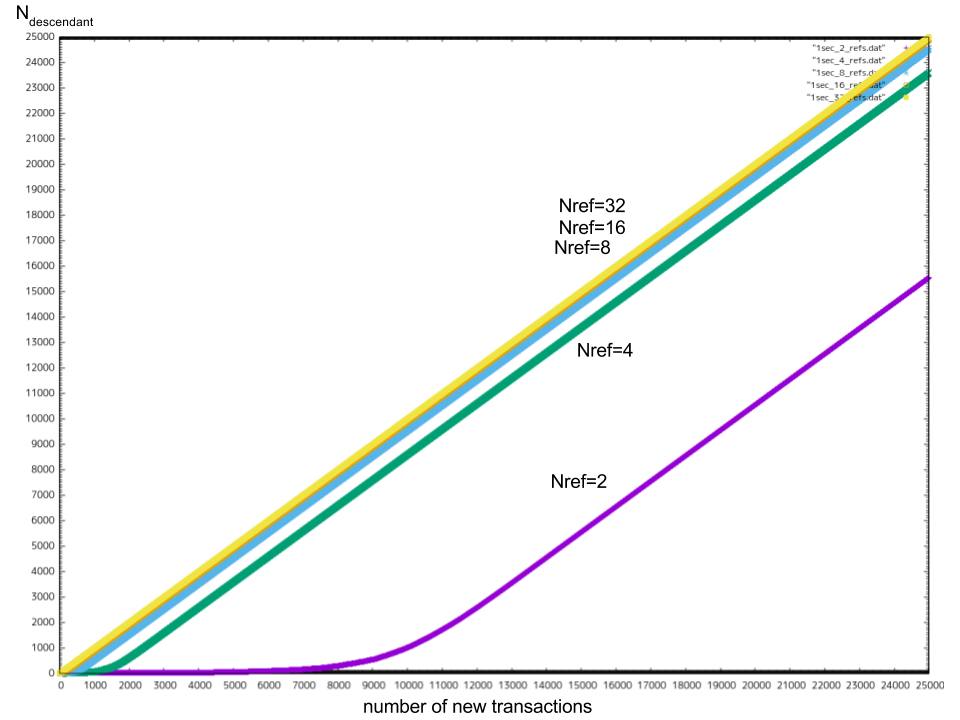
\includegraphics[width=80mm]{1sec_ref.png}
			\caption{\( \lambda_{in}=\) 1 TPS}
		  \label{fig:sec1_ref}
		\end{center}
	 \end{figure}
	
	
	 \begin{figure}[H]
		\begin{center}
			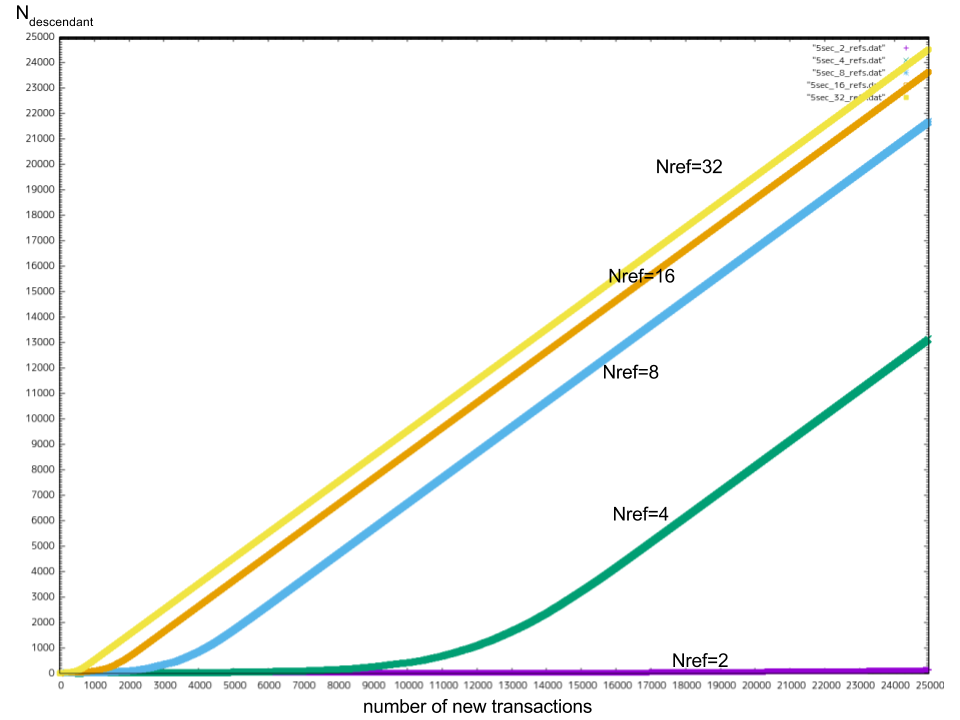
\includegraphics[width=80mm]{5sec_ref.png}
			\caption{ \( \lambda_{in}=\) 5  TPS}
		  \label{fig:sec5_ref}
		\end{center}
	 \end{figure}
	
	 \begin{figure}[H]
		\begin{center}
			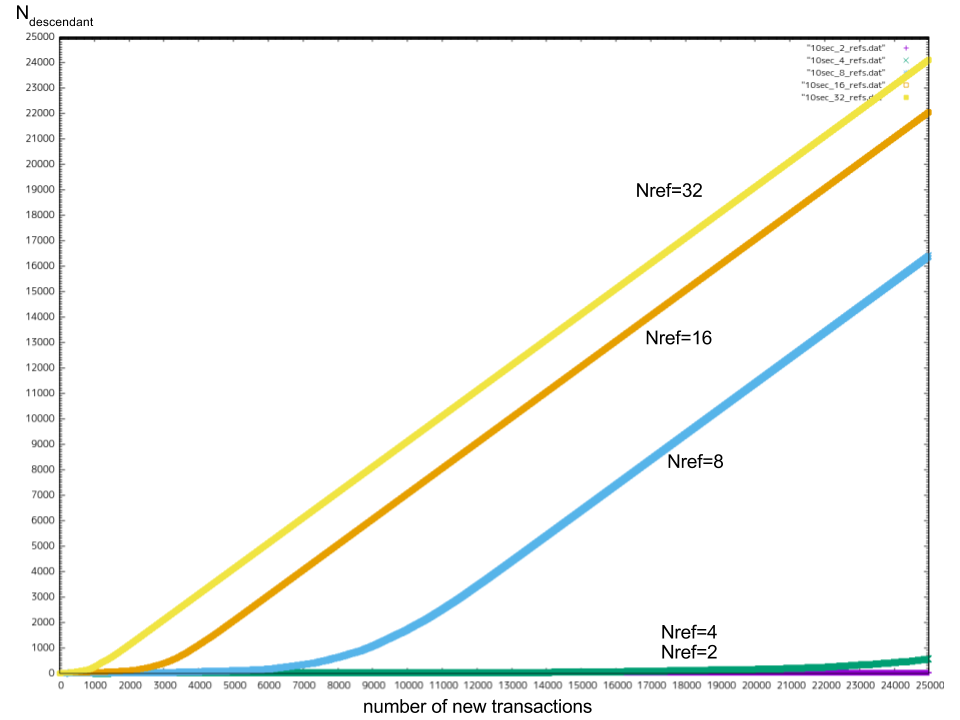
\includegraphics[width=80mm]{10sec_ref.png}
			\caption{ \( \lambda_{in}=\) 10 TPS}
		  \label{fig:sec10_ref}
		\end{center}
	 \end{figure}
	\end{appendices}
	 
	  
	\end{document}
	
